
% this file is called up by thesis.tex
% content in this file will be fed into the main document

%*************************************************************************
%Quote
\begin{savequote}[50mm]
Historical methodology, as I see it, is a product of common sense applied to circumstances. 
\qauthor{Samuel E. Morison}
\end{savequote}
%*************************************************************************

\chapter{N-Body Simulations and Environment Characterization}
\label{cha:N-BodySimulationsAndEnvironmentCharacterization}

% the code below specifies where the figures are stored
\ifpdf
    \graphicspath{{3_overall_methodology/figures/PNG/}{3_overall_methodology/figures/PDF/}{3_overall_methodology/figures/}}
\else
    \graphicspath{{3_overall_methodology/figures/EPS/}{3_overall_methodology/figures/}}
\fi


%*************************************************************************
A brief introduction to N-body simulations 
bla bla bla bla bla bla bla bla bla bla bla bla bla bla bla bla bla bla 
bla bla bla bla bla bla bla bla bla bla bla bla bla bla bla bla bla bla 
bla bla bla bla bla bla bla bla bla bla bla bla bla bla bla bla bla bla 
bla bla bla bla bla bla bla bla bla bla bla bla bla bla bla bla bla bla 
bla bla bla bla bla bla bla bla bla bla bla bla bla bla bla bla bla bla 
%*************************************************************************


%.........................................................................
%Curved Spaces
\begin{figure}[htbp]
	\centering
	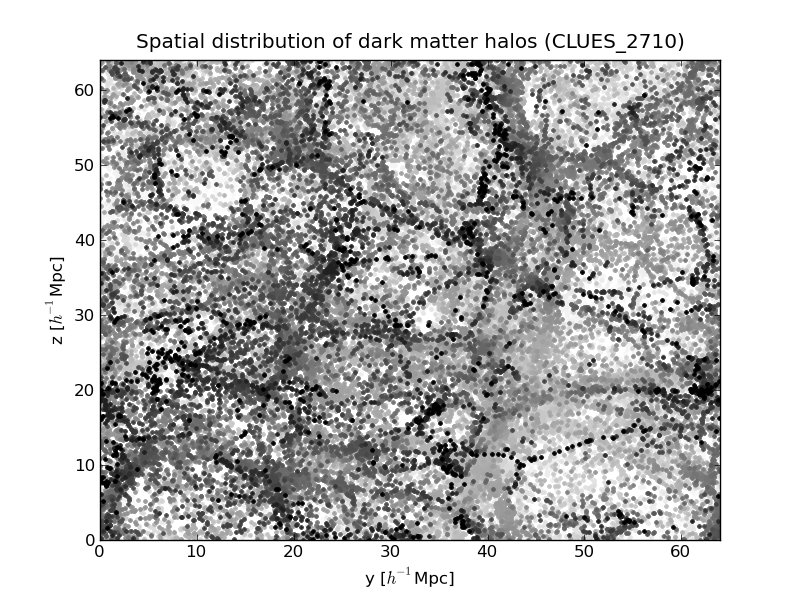
\includegraphics[width=0.9\textwidth]
	{./figures/3_nbody_simulations/Halos_Spatial_Distribution(CLUES_2710).png}
	
	\caption{\small{Halos en simulación CLUES 2710.}}
	
	\label{fig:CurvedSpaces}
\end{figure}
%.........................................................................


%.........................................................................
%Curved Spaces
\begin{figure}[htbp]
	\centering
	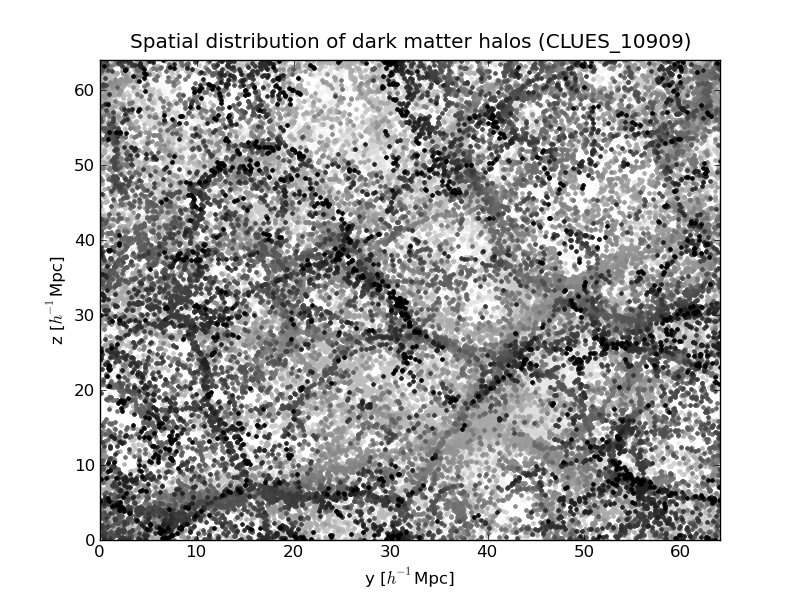
\includegraphics[width=0.9\textwidth]
	{./figures/3_nbody_simulations/Halos_Spatial_Distribution(CLUES_10909).png}
	
	\caption{\small{Halos en simulación CLUES 10909.}}
	
	\label{fig:CurvedSpaces}
\end{figure}
%.........................................................................


%.........................................................................
%Curved Spaces
\begin{figure}[htbp]
	\centering
	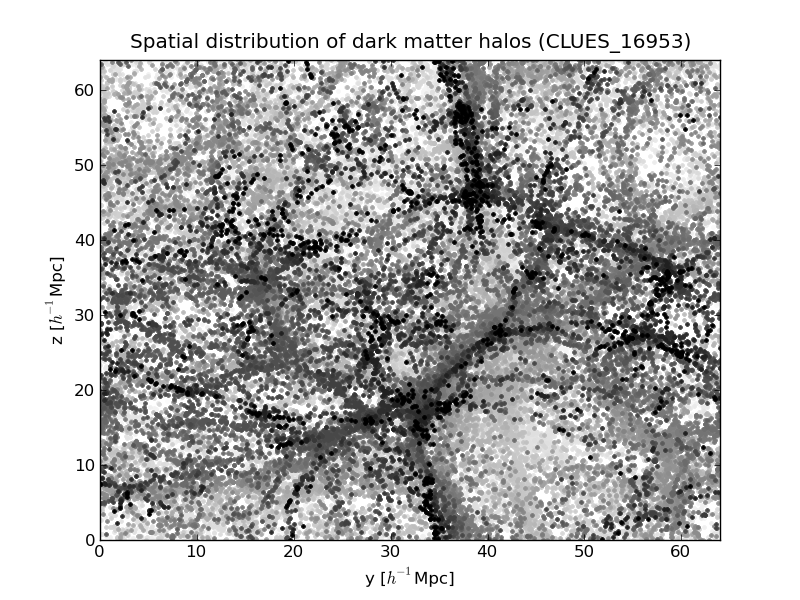
\includegraphics[width=0.9\textwidth]
	{./figures/3_nbody_simulations/Halos_Spatial_Distribution(CLUES_16953).png}
	
	\caption{\small{Halos en simulación CLUES 16953.}}
	
	\label{fig:CurvedSpaces}
\end{figure}
%.........................................................................


%*************************************************************************
%N-body simulations methods
\section{N-body Simulations Methods}
\label{sec:N-bodySimulationsMethods}


	%---------------------------------------------------------------------
	%Direct sum
	\subsection{Direct Sum}
	\label{subsec:DirectSum}
	%---------------------------------------------------------------------


	%---------------------------------------------------------------------
	%Tree codes
	\subsection{Tree Codes}
	\label{subsec:TreeCodes}
	%---------------------------------------------------------------------


	%---------------------------------------------------------------------
	%Hidrodynamical and dark matter simulations
	\subsection{Hidrodynamical and Dark Matter Simulations}
	\label{subsec:HidrodynamicalAndDarkMatterSimulations}
	%---------------------------------------------------------------------


%*************************************************************************




%*************************************************************************
%Types of simulations
\section{Types of Simulations}
\label{sec:Types of Simulations}


	%---------------------------------------------------------------------
	%Constrained simulations (CLUES)
	\subsection{Constrained Simulations (CLUES)}
	\label{subsec:ConstrainedSimulations}
	%---------------------------------------------------------------------


	%---------------------------------------------------------------------
	%Unconstrained simulations (Bolshoi)
	\subsection{Unconstrained Simulations (Bolshoi)}
	\label{subsec:UnconstrainedSimulations}
	%---------------------------------------------------------------------


%*************************************************************************



%*************************************************************************
%Halos detection and sample definitions
\section{Halos Detection and Sample Definitions}
\label{sec:HalosDetectionAndSampleDefinitions}


	%---------------------------------------------------------------------
	%FOF method
	\subsection{FOF Method}
	\label{subsec:FOFMethod}
	%---------------------------------------------------------------------


	%---------------------------------------------------------------------
	%BDM method
	\subsection{BDM Method}
	\label{subsec:BDMMethod}
	%---------------------------------------------------------------------
	
	
	%---------------------------------------------------------------------
	%Sample of pairs to use
	\subsection{Sample of Pairs to Use}
	\label{subsec:SampleOfPairsToUse}
	%---------------------------------------------------------------------
	
	
	%---------------------------------------------------------------------
	%Pair finder method
	\subsection{Pair Finder Method}
	\label{subsec:PairFinderMethod}
	%---------------------------------------------------------------------


%*************************************************************************




%*************************************************************************
%Environment Characterization
\section{Environment Characterization}
\label{sec:EnvironmentCharacterization}


	%---------------------------------------------------------------------
	%The T-web Method
	\subsection{The T-web Method}
	\label{subsec:TheT-webMethod}
	%---------------------------------------------------------------------


	%---------------------------------------------------------------------
	%The V-web Method
	\subsection{The V-web Method}
	\label{subsec:TheV-webMethod}
	%---------------------------------------------------------------------


%*************************************************************************